\documentclass[a4j,dvipdfmx]{jsarticle}
\usepackage{amsmath,amssymb}
\usepackage{siunitx}
\usepackage{bm}

\usepackage[subrefformat=parens]{subcaption}

\usepackage[margin=15truemm,nohead]{geometry}
\usepackage{qexam}

\usepackage{tikz}
\usepackage{tikz-3dplot}
\usetikzlibrary{calc}
\usetikzlibrary{angles, quotes}

\renewcommand{\div}{{\rm div}\hspace{1mm}}
\newcommand{\grad}{{\rm grad}\hspace{1mm}}
\newcommand{\rot}{{\rm rot}\hspace{1mm}}

\begin{document}
    \part*{理学同好会 ベクトル解析 テスト2 解答}
    \color{red}
    以下に解答例を述べる. 計算ミス等あったら教えてください.

    \question{問1}
        \begin{qparts}
            \qpart 球面座標は下図のようにとった. これらはあくまで例であり, 別のパラメータを選ぶと別の表式が得られることも注意しておく.
            \begin{qlist}
                \qitem $\bm{r}(\phi,\theta)=[a\sin\theta\cos\phi,a\sin\theta\sin\phi,a\cos\theta]$ 

                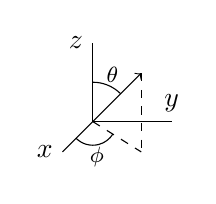
\begin{tikzpicture}
                    \coordinate (A) at (1,0,1);
                    \coordinate (P) at (1,1,1);
                    \coordinate (O) at (0,0,0);
                    \coordinate (X) at (0,0,1);
                    \coordinate (Y) at (0,1,0);
                    \draw[->] (O) -- (P);
                    \draw (O) -- (1,0,0); 
                    \draw (O) -- (X); 
                    \draw (O) -- (Y); 
                    \draw[dashed] (P) -- (A);
                    \draw[dashed] (O) -- (A);
                    \draw pic["$\theta$", draw, font=\footnotesize, angle eccentricity=1.3, angle radius=0.5cm] {angle=P--O--Y};
                    \draw pic["$\phi$", draw, font=\footnotesize, angle eccentricity=1.5, angle radius=0.3cm] {angle=X--O--A};
                    \node[left] at (0,0,1) {$x$};
                    \node[left] at (0,1,0) {$z$};
                    \node[above] at (1,0,0) {$y$};
                \end{tikzpicture}
                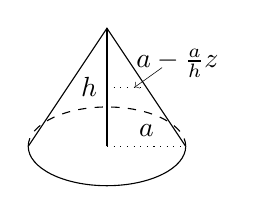
\begin{tikzpicture}
                    \draw (4,0) arc[x radius=1, y radius=0.5, start angle=0, end angle=-180];
                    \draw[dashed] (2,0) arc[x radius=1, y radius=0.5, start angle=-180, end angle=-360];
                    \draw (2,0) -- (3,1.5) -- (4,0);
                    \draw (3,0) -- (3,1.5);
                    \draw[dotted] (3,0) -- (4,0);
                    \node[above] at (3.5,0) {$a$};
                    \node[left] at (3,0.75) {$h$};
                    \draw[dotted] (3,0.75) -- (3.5,0.75);
                    \node[above right] at (3.25,0.75) {$a-\frac{a}{h}z$};
                    \draw[->,very thin] (3.7,1) -- (3.35,0.75);
                \end{tikzpicture}
                \qitem $\bm{r}(\theta,z)=[\left(a-\frac{a}{h}z\right)\cos \phi,(a-\frac{a}{h}z)\sin\phi,z]\quad (0\leq \phi\leq 2\pi,0\leq z\leq h)$
                \qitem $\bm{r}(x,y)=[x,y,f(x,y)]$
                \qitem $\bm{r}(u,v) = [a\cosh u\cos v,b\cosh u\sin v,c\sinh u]$
            \end{qlist}
            \qpart 曲面は, $\bm{r}(\phi,u)=[u\cos\phi,u\sin\phi,\sqrt{a^2-u^2}]$と書ける. $u$が長さの変わる半径とイメージできれば, これは一般の回転体でも使えることわかる. \footnote{一般に, 曲線$z=f(u)$をz軸回りに回転させてできる回転面は$\bm{r}(\phi,u)=[u\cos\phi,u\sin\phi,f(u)]$と書ける.}
            \begin{qlist}
                \qitem $\bm{r}_\phi=[-u\sin\phi,u\cos\phi,0],\bm{r}_u=[\cos\phi,\sin\phi,\frac{-u}{\sqrt{a^2-u^2}}]$より\\
                $E=\bm{r}_\phi^2=u^2,F=\bm{r}_\phi\cdot\bm{r}_u=0,G=\bm{r}_u^2=1+\frac{u^2}{a^2-u^2}=\frac{a^2}{a^2-u^2}$
                \qitem $dS=\sqrt{EG-F^2}d\phi du=\frac{au}{\sqrt{a^2-u^2}}d\phi du$
                \qitem $\int_S dS=\int_0^a du\int_0^{2\pi} \frac{au}{\sqrt{a^2-u^2}}d\phi=2\pi a\int_{0}^{a}\left\{-\sqrt{a^2-u^2}\right\}'du=2\pi a^2$で, 球全体はこれを二倍する.
                \qitem 定義より$\bm{n}=\frac{\bm{r}_\phi\times\bm{r}_u}{|\bm{r}_\phi\times\bm{r}_u|}=\frac{\sqrt{a^2-u^2}}{au}(\bm{r}_\phi\times\bm{r}_u)=\frac{\sqrt{a^2-u^2}}{au}[-\frac{u^2}{\sqrt{a^2-u^2}}\cos\phi,-\frac{u^2}{\sqrt{a^2-u^2}}\sin\phi,-u]$\\
                $=[-\frac{u}{a}\cos\phi,-\frac{u}{a}\sin\phi,-\frac{\sqrt{a^2-u^2}}{a}]$ \label{q:円の法線}
                \qitem $\bm{r}_{\phi\phi}=[-u\cos\phi,-u\sin\phi,0],\bm{r}_{\phi u}=[-\sin\phi,-\cos\phi,0],\bm{r}_{uu}=\left[0,0,\frac{-a^2}{(a^2-u^2)^{\frac{3}{2}}}\right]$より\\
                $L=\bm{n}\cdot\bm{r}_{\phi\phi}=\frac{u^2}{a^2},M=\bm{n}\cdot\bm{r}_{\phi u}=0,N=\bm{n}\cdot\bm{r}_{uu}=\frac{a}{a^2-u^2}$
                \qitem $K=\frac{LM-N^2}{EG-F^2}=\frac{1}{a},H=\frac{1}{2}\frac{GL+EN-2FM}{EG-F^2}=\frac{1+a}{2a^2}$
            \end{qlist}
            \qpart 以下は簡単な証明問題である.
            \begin{qlist}
                \qitem $\bm{r}$と$\bm{n}$が平行であることを示せばよい. 先ほどの\qref{q:円の法線}から$\bm{n}=-\frac{1}{a}\bm{r}$となることを示せ.
                \qitem 
                \begin{equation*}
                    \bm{r}_u\times\bm{r}_v = \begin{vmatrix}
                        \bm{i} & \bm{j} & \bm{k} \\
                        x_u & y_u & z_u \\
                        x_v & y_v & z_v
                        \end{vmatrix}=\left[
                            \begin{vmatrix}
                                y_u & z_u \\
                                y_v & z_v
                            \end{vmatrix},
                            -\begin{vmatrix}
                                x_u & z_u \\
                                x_v & z_v
                            \end{vmatrix},
                            \begin{vmatrix}
                                x_u & y_u \\
                                x_v & y_v
                            \end{vmatrix}
                        \right]=\left[\frac{\partial (y,z)}{\partial (u,v)},\frac{\partial (z,x)}{\partial (u,v)},\frac{\partial (x,y)}{\partial (u,v)}\right]              
                \end{equation*}
                より示される. ここで$\displaystyle
                -\begin{vmatrix}
                    x_u & z_u \\
                    x_v & z_v
                \end{vmatrix}=
                \begin{vmatrix}
                    z_u & x_u \\
                    z_v & x_v
                \end{vmatrix}$を用いた.
            \end{qlist}
            \clearpage
            \qpart IIの手順のように計算する.
            \begin{align*}
                \bm{r}_u&=\left[k\cos u\cos v,k\cos u\sin v,\frac{k}{2\sin\frac{u}{2}\cos\frac{u}{2}}-k\sin u\right]=\left[k\cos u\cos v,k\cos u\sin v,k\left(\frac{1}{\sin u}-\sin u\right)\right]\\
                \bm{r}_v&=\left[k\sin u\sin v,k\sin u\cos v,0\right]
            \end{align*}
            だから
            \begin{align*}
                E&=\bm{r}_u^2=k^2\cos^2 u + \frac{k^2}{\sin^2 u}-2k^2+k^2\sin^2 u=\frac{k^2}{\sin^2 u}-k^2=k^2\frac{\cos^2 u}{\sin^2 u}\\
                F&=\bm{r}_u\cdot \bm{r}_v = 0\\
                G&=\bm{r}_v^2=k^2\sin^2 u
            \end{align*}
            単位法線ベクトルは
            \begin{align*}
                \bm{n}&=\frac{\bm{r}_u\times\bm{r}_v}{\sqrt{EG-F^2}}=\frac{1}{k^2\sqrt{\cos^2u}}[k^2(\sin^2u\cos v-\cos v),-k^2(\sin v-\sin^2 u\sin v),k^2\cos u\sin u]\\
                      &=\frac{1}{k^2\sqrt{\cos^2u}}[-k^2\cos^2u\cos v,-k^2\cos^2u\sin v,k^2\cos u\sin u]\\
                      &=[-\cos u\cos v,-\cos u\sin v,\sin u]
            \end{align*}
            となる.\footnote{鋭い人なら,$u$の範囲から$\sqrt{\cos^2 u}=|\cos u|$とすべきではと思ったかもしれない. この指摘は完全に正しい. 本来法線ベクトルは連続的に変化するように取るべきだから, 一方で曲面の内側, もう一方で外側に取るなどは好ましくない. ただ今回の場合はどちらの符号を選んだとしても
            Gauss曲率$K$の$LN$の部分で打ち消すから`たまたま'問題なかっただけである.}
            曲面の二回微分を求めると
            \begin{align*}
                \bm{r}_{uu}&=\left[-k\sin u\cos v,-k\sin u\sin v,k\left(-\frac{\cos u}{\sin^2 u}-\cos u\right)\right]\\
                           &=\left[-k\sin u\cos v,-k\sin u\sin v,-k\cos u\left(1+\frac{1}{\sin^2 u}\right)\right]\\
                \bm{r}_{uv}&=\left[-k\cos u\sin v,k\cos u\cos v,0\right]\\
                \bm{r}_{vv}&=\left[-k\sin u\cos v,-k\sin u\sin v,0\right]
            \end{align*}
            だから, 第2基本量は
            \begin{align*}
                L&=\bm{n}\cdot\bm{r}_{uu}=k\cos u\sin u-k\cos u\left(\sin u+\frac{1}{\sin u}\right)=-k\frac{\cos u}{\sin u}\\
                M&=\bm{n}\cdot \bm{r}_{uv} = 0\\
                N&=\bm{n}\cdot\bm{r}_{vv}=k\cos u\sin u
            \end{align*}
            これより, Gauss曲率を求めると
            \begin{equation*}
                K=\frac{LN-M^2}{EG-F^2}=\frac{-k^2\cos^2u}{k^4\cos^2u}=-\frac{1}{k^2}
            \end{equation*}
            となり, 負の一定値であることがわかる.
        \end{qparts}
    \clearpage

    \question{問2}
        \begin{qparts}
            \qpart 概形は以下のとおりである. 図の作成にはGeoGebra\footnote{https://www.geogebra.org/graphing?lang=ja}を用いた.
            \begin{figure}[h]
                \begin{minipage}[t]{.3\textwidth}
                    \centering
                    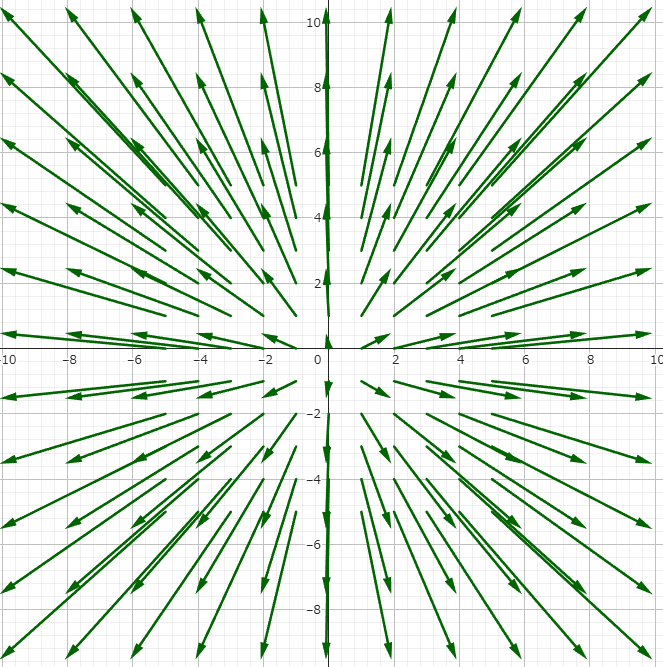
\includegraphics[scale=0.20]{img/vector_field1.png}
                    \subcaption{$\bm{v}=[x,y]$}
                \end{minipage}
                \begin{minipage}[t]{.3\textwidth}
                    \centering
                    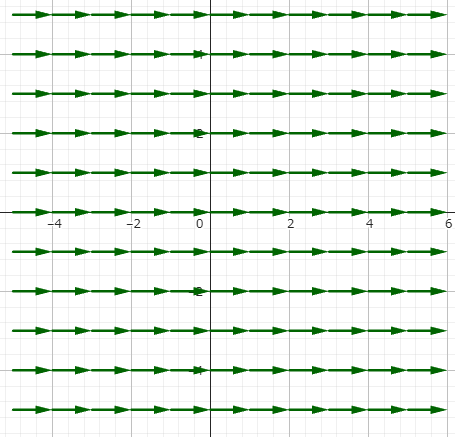
\includegraphics[scale=0.35]{img/vector_field2.png}
                    \subcaption{$\bm{v}=[1,0]$}
                \end{minipage}
                \begin{minipage}[t]{.3\textwidth}
                    \centering
                    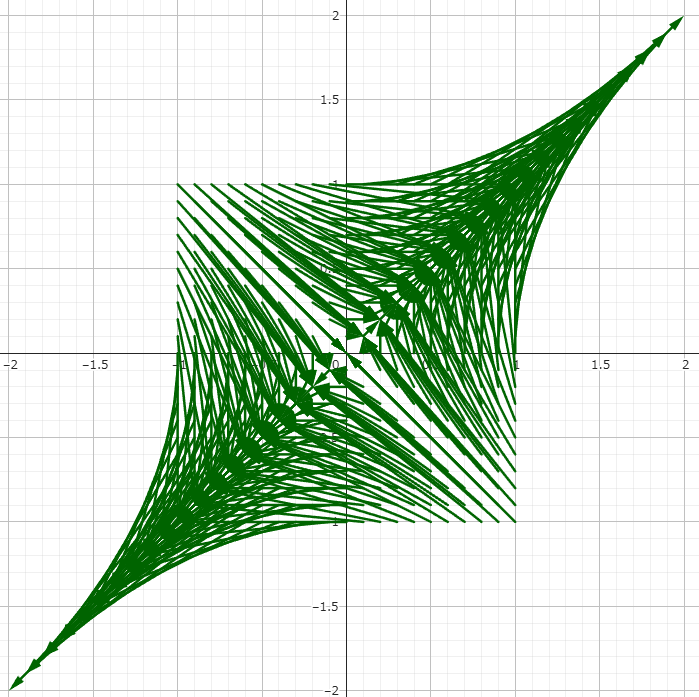
\includegraphics[scale=0.25]{img/vector_field3.png}
                    \subcaption{$\bm{v}=[y,x]$}
                \end{minipage}
                \caption{各ベクトル場}
            \end{figure}
            \qpart 
            \begin{qlist}
                \setcounter{enumi}{3}
                \qitem $\grad U = [0,mg]$
                \qitem $\grad U = [2,1]$
                \qitem $\grad U = [0,mg,0]$
                \qitem 普通に計算してもよいが, これは電位の式だから
                $\displaystyle \grad V(x,y,z)=-\frac{Q}{4\pi\varepsilon_0r^3}\bm{r}\quad (\bm{r}=[x,y,z],r=|\bm{r}|)$
            \end{qlist}
            \qpart 
            \begin{qlist}
                \qitem $\div\bm{v}=0,\rot\bm{v}=\bm{0}$
                \qitem $\div\bm{v}=2x+1,\rot\bm{v}=[1,0,1]$
                \qitem $\displaystyle \div\bm{v}=\frac{\sqrt{x^2+y^2}-\frac{x^2}{\sqrt{x^2+y^2}}}{x^2+y^2}+\frac{\sqrt{x^2+y^2}-\frac{y^2}{\sqrt{x^2+y^2}}}{x^2+y^2}=\frac{y^2+x^2}{(x^2+y^2)^{\frac{3}{2}}}=\frac{1}{\sqrt{x^2+y^2}}$\\
                $\displaystyle
                    \rot \bm{v}=\begin{vmatrix}
                        \bm{i} & \bm{j} & \bm{k} \\
                        \partial_x & \partial_y & \partial_z \\
                        \frac{x}{\sqrt{x^2+y^2}} & \frac{y}{\sqrt{x^2+y^2}} & 0
                    \end{vmatrix}=\left[0,0,-\frac{2xy}{(x^2+y^2)^{\frac{3}{2}}}\right]
                $
            \end{qlist}
            \qpart ノートに書いてあることと重複するが, 一応述べる.
            \begin{qlist}
                \qitem $\div \grad f = \div\partial_i f=\partial_i \partial_i f=\nabla^2 f$
                \qitem $(\rot \grad f)_k = (\rot\partial_jf)_k=\varepsilon_{kij}\partial_i\partial_j f$で, $f_x,f_y,f_z$の連続性を認めれば$\partial_i\partial_j f=\partial_j\partial_i f$だから$0$となる.
                \qitem $\div \rot\bm{v}=\partial_k (\varepsilon_{kij}\partial_iv_j)=\varepsilon_{kij}\partial_k\partial_iv_j=\varepsilon_{jki}\partial_k\partial_iv_j$より前問同様$0$となる.
                \qitem $(\rot \rot\bm{v})_k=\varepsilon_{kij}\partial_i(\rot\bm{v})_j=\varepsilon_{kij}\partial_i\varepsilon_{jlm}\partial_lv_m=\varepsilon_{kij}\varepsilon_{jlm}\partial_i\partial_lv_m=\varepsilon_{jki}\varepsilon_{jlm}\partial_i\partial_lv_m$\\
                ここで$\varepsilon_{jki}\varepsilon_{jlm}=\delta_{kl}\delta_{im}-\delta_{km}\delta_{il}$だから$\varepsilon_{jki}\varepsilon_{jlm}\partial_i\partial_lv_m=(\delta_{kl}\delta_{im}-\delta_{km}\delta_{il})\partial_i\partial_lv_m=\partial_m\partial_kv_m-\partial_l\partial_lv_k$\\
                一項目は微分の順序を入れ替えれば$\grad\div\bm{v}$であり, 二項目は$\nabla^2\bm{v}$だから, 証明が完了した. 
            \end{qlist}
        \end{qparts}
    \clearpage
    \question{問3}
        \begin{qparts}
            \qpart $\bm{F}=[y^2,x+y^2]$の場合は以下の通り.
            \begin{qlist}
                \qitem $\int_{C_1}\bm{F}\cdot d\bm{r}=0$
                \qitem $\int_{C_2}\bm{F}\cdot d\bm{r}=\int_{0}^{4}(4+y^2)dy=\frac{112}{3}$
                \qitem $\int_{C_1+C_2}=\int_{C_1}+\int_{C_2}=\frac{112}{3}$
                \qitem $dy=\frac{1}{2}xdx$より$\int_{C_3}\bm{F}\cdot d\bm{r}=\int_0^4\left\{\frac{x^4}{16}dx+\left(x+\frac{x^4}{16}\right)\frac{x}{2}dx\right\}=\int_0^4\left(\frac{x^5}{32}+\frac{x^4}{16}+\frac{x^2}{2}\right)dx=\frac{224}{5}$
                \qitem $y^2=4x$より$dx=\frac{1}{2}ydy$だから$\int_{C_4}\bm{F}\cdot d\bm{r}=\int_0^4\left\{\frac{1}{2}y^3+\frac{5}{4}y^2\right\}dy=\frac{320}{3}$
            \end{qlist}
            $\bm{F}=[ax+by,bx+cy]$のときについて考える. もちろん普通に計算してもよいが, $\bm{F}\cdot d\bm{r}=(ax+by)dx+(bx+cy)dy=d\left(\frac{a}{2}x^2\right)+d(bxy)+d\left(\frac{c}{2}y^2\right)=d\left(\frac{ax^2+2bxy+cy^2}{2}\right)$より\\
            $\int_{C_1} = 8a,\int_{C_2}=8(a+2b+c)-8a=8(2b+c)$であり, $\int_{C_1+C_2}=\int_{C_3}=\int_{C_4}=8(a+2b+c)$
        \qpart 積分記号下が$\grad (xyz)\cdot d\bm{r}$であることより示される.
        \qpart 半径を$a$とおく.
            \begin{equation*}
                \oint_\Gamma \frac{x^3-3xy^2}{(x^2+y^2)^2}dx=\int_{-a}^{a} \frac{x^3-3x(a^2-x^2)}{a^4}dx=\int_{-a}^{a}\frac{1}{a^4}(4x^3-3a^2x)dx=0
            \end{equation*}
        \qpart Gaussの定理を用いる.
            \begin{qlist}
                \qitem $\displaystyle \iint_S \bm{F}\cdot\bm{n}dS=\iiint_V (2x+2y+2z)dxdydz=\int_{-1}^{1}dz\int_{-1}^{1}dy\int_{-1}^{1}(2x+2y+2z)dx=0$
                \qitem $\displaystyle \iint_S\bm{F}\cdot\bm{n}dS=\iiint3dxdydz=3\cdot 2^2\pi\cdot 5 = 60\pi$
                \qitem $\bm{F}=[x^3,y^3,z^3],\bm{n}=[x,y,z]$として, $\displaystyle \iint_S \bm{F}\cdot\bm{n}dS=3\iiint_{x^2+y^2+z^2\leq 1}(x^2+y^2+z^2)dxdydz$\\
                $\displaystyle=3\int_{0}^{2\pi}d\phi\int_{0}^{\pi}d\theta\int_{0}^{1}r^2\cdot r^2\sin^2\theta dr=\frac{12}{5}\pi$\label{q:Gauss直接できないやつ}
            \end{qlist}
            特に, \qref{q:Gauss直接できないやつ}については自分でベクトル場と法線ベクトルを設定する必要があるから注意. 条件を満たすベクトル場は無限に選べるから, 適当なものを選ばないと
            計算が煩雑になる.
        \qpart 
            \begin{qlist}
                \qitem 質量$m$の質点と単位質量の質点を結ぶ直線状に働き, 吸引力だから方向は$-\frac{\bm{r}}{r}$で, 大きさは$|\bm{F}|=F$となっているから.
                \qitem $S$が半径$r$の球表面だから
                    \begin{equation*}
                        \iint_S \bm{F}\cdot d\bm{S} =\iint_S\bm{F}\cdot \frac{\bm{r}}{r}dS=-\frac{Gm}{r^2}\iint_S dS=-\frac{Gm}{r^2}\cdot 4\pi r^2 =-4\pi Gm
                    \end{equation*}
            \end{qlist}
        \qpart $\arctan x$の導関数がわかれば解ける問題.
            \begin{qlist}
                \qitem $\partial_x \theta=-\frac{y}{x^2+y^2},\partial_y \theta=\frac{x}{x^2+y^2}$
                \qitem $d\theta=-\frac{y}{x^2+y^2}dx+\frac{x}{x^2+y^2}dy$
                \qitem $\bm{F}\cdot d\bm{r}=d\theta$だから積分$\oint_C \bm{F}\cdot d\bm{r}=\oint_C d\theta$は$C$が原点回りを何rad回ったかを表す.
                これを$2\pi$で割れば, 何回回ったかが求められる. これは$\arctan$が多価関数であることに起因する.
                図を描くとイメージしやすい.
            \end{qlist}
        \end{qparts}
    \color{black}
    \hrulefill  以上 \hrulefill\\
    解く目安:1時間30分程度.\\
    今回はGreenの定理, Stokesの定理に関する設問を一つも用意しなかった. Greenの定理は来年の複素解析(予定)でも必要となるのでしっかり理解しておこう. 最後に, 問題数を考えて入れなかったStokesの定理に関する問題をあげて終わる.\\
    \fbox{$\bm{F}=[y,-x,2x^3y^2], S=\{x^2+y^2+3z^2=1,z\leq0\}$のとき, $\iint_S\rot\bm{F}\cdot\bm{n}dS$を求めよ.ただし, $S$は球面の外側を表とする.}
    答えは$2\pi$である. ($z\leq 0$だから通常の円周と向きが反対になることに注意.)

\end{document}